\documentclass{article}

\usepackage{a4}
\usepackage{amsmath}
\usepackage{amssymb}
\usepackage{ctex}
\usepackage{booktabs}
\usepackage{graphicx}
\usepackage{subfigure}
\usepackage{subcaption}
\usepackage{float}
\usepackage{hyperref}
\usepackage{xurl}
\usepackage{enumitem}
\usepackage{array}
\usepackage{longtable}
\usepackage{multirow}
\usepackage{fvextra}

\hypersetup{colorlinks=true,linkcolor=black,urlcolor=blue,citecolor=black}
\setlist[itemize]{nosep,leftmargin=1.8em}
\setlist[enumerate]{nosep,leftmargin=1.8em}
\captionsetup{font=small}
\RecustomVerbatimEnvironment{verbatim}{Verbatim}{
  breaklines=true,
  breakanywhere=true,
  fontsize=\small
}

\title{计算机组成原理 \\ 实验3 寄存器堆实现与改造}
\author{鲁昕宁 2414015}
\date{\today}

\begin{document}

\maketitle
\begin{center}
    \url{https://github.com/SidneyLu/Computer-Organization-and-Design-NKU-CS/tree/master/lab3}
\end{center}

\newpage

\section{实验目标}
参考实验指导手册第三次的寄存器实验，完成对寄存器堆的改进：
\begin{enumerate}
    \item 原来的写使能（wen）信号扩展成2位，分别控制写入wdata的高16位和低16位。
    \item 增加一个专用寄存器，用来存储1号寄存器和2号寄存器中数据之和。
\end{enumerate}

\section{实验原理}
\begin{figure}[H]
    \centering
    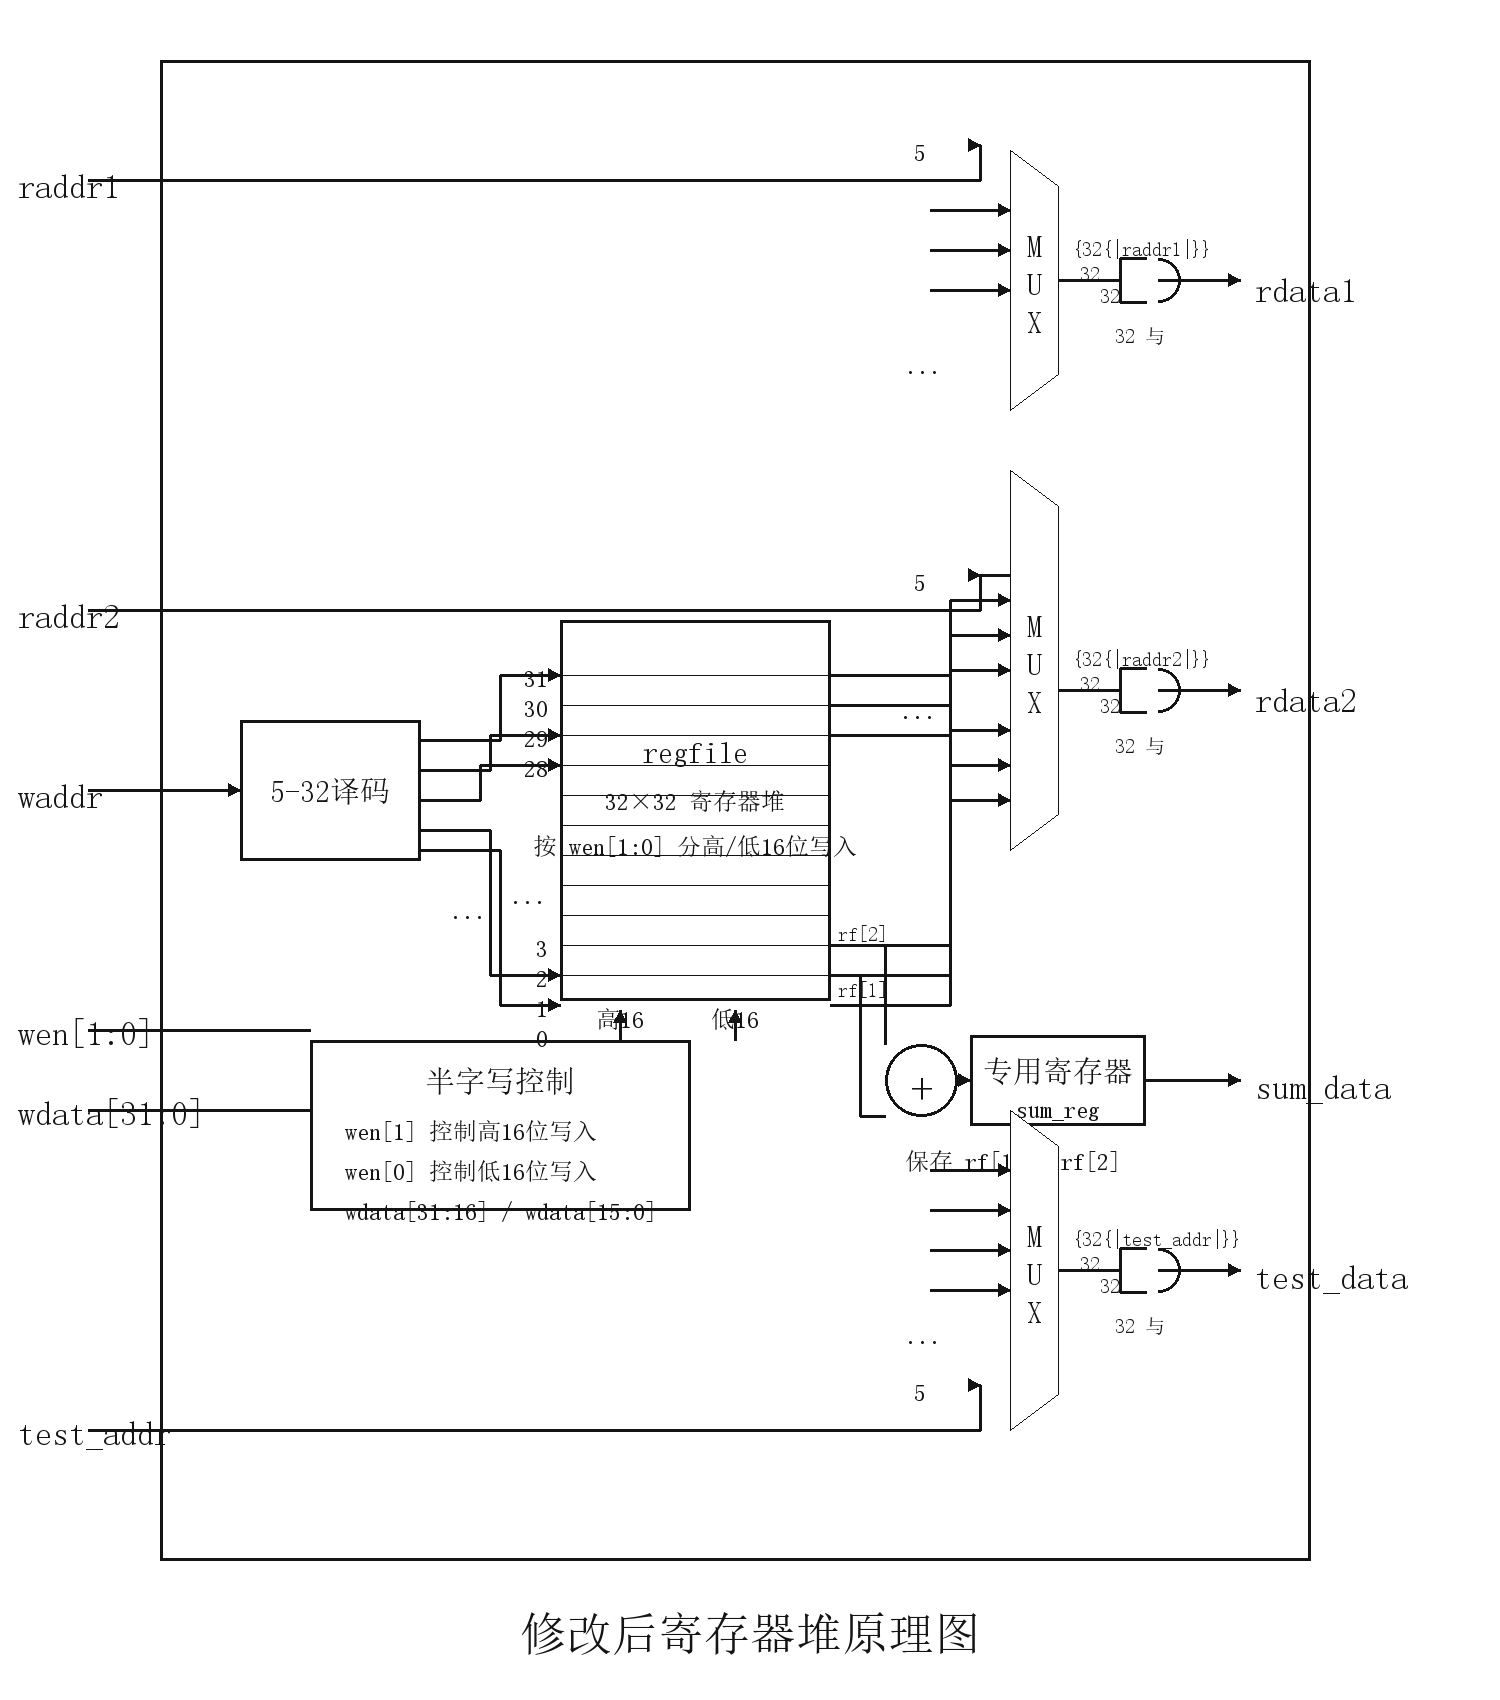
\includegraphics[width=0.8\textwidth]{modified_regfile_schematic.png}
    \label{fig:modified}
\end{figure}


\section{实验过程}

\subsection{源码}
\subsubsection{regfile.v}
\begin{verbatim}
`timescale 1ns / 1ps
//*************************************************************************
//   > 文件名: regfile.v
//   > 描述  ：寄存器堆模块，同步写，异步读
//   > 作者  : LOONGSON
//   > 日期  : 2016-04-14
//*************************************************************************
module regfile(
    input             clk,
    input      [1 :0] wen,
    input      [4 :0] raddr1,
    input      [4 :0] raddr2,
    input      [4 :0] waddr,
    input      [31:0] wdata,
    output reg [31:0] rdata1,
    output reg [31:0] rdata2,
    input      [4 :0] test_addr,
    output reg [31:0] test_data,
    output reg [31:0] sum_data
    );
    reg [31:0] rf[31:0];
    integer i;

    function [31:0] merge_wdata;
        input [31:0] old_data;
        input [31:0] new_data;
        input [1 :0] wen_bits;
        begin
            merge_wdata = old_data;
            if (wen_bits[0])
                merge_wdata[15:0]  = new_data[15:0];
            if (wen_bits[1])
                merge_wdata[31:16] = new_data[31:16];
        end
    endfunction

    initial begin
        for (i = 0; i < 32; i = i + 1) begin
            rf[i] = 32'd0;
        end
        sum_data = 32'd0;
    end
     
    // three ported register file
    // read two ports combinationally
    // write third port on rising edge of clock
    // register 0 hardwired to 0

    always @(posedge clk)
    begin
        if (|wen && waddr != 5'd0) 
        begin
            rf[waddr] <= merge_wdata(rf[waddr], wdata, wen);
        end
        sum_data <= ((waddr == 5'd1) ? merge_wdata(rf[1], wdata, wen) : rf[1]) +
                    ((waddr == 5'd2) ? merge_wdata(rf[2], wdata, wen) : rf[2]);
    end
     
    //读端口1
    always @(*)
    begin
        case (raddr1)
            5'd1 : rdata1 <= rf[1 ];
            5'd2 : rdata1 <= rf[2 ];
            5'd3 : rdata1 <= rf[3 ];
            5'd4 : rdata1 <= rf[4 ];
            5'd5 : rdata1 <= rf[5 ];
            5'd6 : rdata1 <= rf[6 ];
            5'd7 : rdata1 <= rf[7 ];
            5'd8 : rdata1 <= rf[8 ];
            5'd9 : rdata1 <= rf[9 ];
            5'd10: rdata1 <= rf[10];
            5'd11: rdata1 <= rf[11];
            5'd12: rdata1 <= rf[12];
            5'd13: rdata1 <= rf[13];
            5'd14: rdata1 <= rf[14];
            5'd15: rdata1 <= rf[15];
            5'd16: rdata1 <= rf[16];
            5'd17: rdata1 <= rf[17];
            5'd18: rdata1 <= rf[18];
            5'd19: rdata1 <= rf[19];
            5'd20: rdata1 <= rf[20];
            5'd21: rdata1 <= rf[21];
            5'd22: rdata1 <= rf[22];
            5'd23: rdata1 <= rf[23];
            5'd24: rdata1 <= rf[24];
            5'd25: rdata1 <= rf[25];
            5'd26: rdata1 <= rf[26];
            5'd27: rdata1 <= rf[27];
            5'd28: rdata1 <= rf[28];
            5'd29: rdata1 <= rf[29];
            5'd30: rdata1 <= rf[30];
            5'd31: rdata1 <= rf[31];
            default : rdata1 <= 32'd0;
        endcase
    end
    //读端口2
    always @(*)
    begin
        case (raddr2)
            5'd1 : rdata2 <= rf[1 ];
            5'd2 : rdata2 <= rf[2 ];
            5'd3 : rdata2 <= rf[3 ];
            5'd4 : rdata2 <= rf[4 ];
            5'd5 : rdata2 <= rf[5 ];
            5'd6 : rdata2 <= rf[6 ];
            5'd7 : rdata2 <= rf[7 ];
            5'd8 : rdata2 <= rf[8 ];
            5'd9 : rdata2 <= rf[9 ];
            5'd10: rdata2 <= rf[10];
            5'd11: rdata2 <= rf[11];
            5'd12: rdata2 <= rf[12];
            5'd13: rdata2 <= rf[13];
            5'd14: rdata2 <= rf[14];
            5'd15: rdata2 <= rf[15];
            5'd16: rdata2 <= rf[16];
            5'd17: rdata2 <= rf[17];
            5'd18: rdata2 <= rf[18];
            5'd19: rdata2 <= rf[19];
            5'd20: rdata2 <= rf[20];
            5'd21: rdata2 <= rf[21];
            5'd22: rdata2 <= rf[22];
            5'd23: rdata2 <= rf[23];
            5'd24: rdata2 <= rf[24];
            5'd25: rdata2 <= rf[25];
            5'd26: rdata2 <= rf[26];
            5'd27: rdata2 <= rf[27];
            5'd28: rdata2 <= rf[28];
            5'd29: rdata2 <= rf[29];
            5'd30: rdata2 <= rf[30];
            5'd31: rdata2 <= rf[31];
            default : rdata2 <= 32'd0;
        endcase
    end
     //调试端口，读出寄存器值显示在触摸屏上
    always @(*)
    begin
        case (test_addr)
            5'd1 : test_data <= rf[1 ];
            5'd2 : test_data <= rf[2 ];
            5'd3 : test_data <= rf[3 ];
            5'd4 : test_data <= rf[4 ];
            5'd5 : test_data <= rf[5 ];
            5'd6 : test_data <= rf[6 ];
            5'd7 : test_data <= rf[7 ];
            5'd8 : test_data <= rf[8 ];
            5'd9 : test_data <= rf[9 ];
            5'd10: test_data <= rf[10];
            5'd11: test_data <= rf[11];
            5'd12: test_data <= rf[12];
            5'd13: test_data <= rf[13];
            5'd14: test_data <= rf[14];
            5'd15: test_data <= rf[15];
            5'd16: test_data <= rf[16];
            5'd17: test_data <= rf[17];
            5'd18: test_data <= rf[18];
            5'd19: test_data <= rf[19];
            5'd20: test_data <= rf[20];
            5'd21: test_data <= rf[21];
            5'd22: test_data <= rf[22];
            5'd23: test_data <= rf[23];
            5'd24: test_data <= rf[24];
            5'd25: test_data <= rf[25];
            5'd26: test_data <= rf[26];
            5'd27: test_data <= rf[27];
            5'd28: test_data <= rf[28];
            5'd29: test_data <= rf[29];
            5'd30: test_data <= rf[30];
            5'd31: test_data <= rf[31];
            default : test_data <= 32'd0;
        endcase
    end
endmodule
\end{verbatim}

\subsubsection{regfile\_display.v}
\begin{verbatim}
//*************************************************************************
//   > 文件名: regfile_display.v
//   > 描述  ：寄存器堆显示模块，调用FPGA板上的IO接口和触摸屏
//   > 作者  : LOONGSON
//   > 日期  : 2016-04-14
//*************************************************************************
module regfile_display(
    //时钟与复位信号
    input clk,
    input resetn,    //后缀"n"代表低电平有效

    //拨码开关，用于产生写使能和选择输入数
    input [1:0] wen,
    input [1:0] input_sel,

    //led灯，用于指示写使能信号，和正在输入什么数据
    output [1:0] led_wen,
    output led_waddr,    //指示输入写地址
    output led_wdata,    //指示输入写数据
    output led_raddr1,   //指示输入读地址1
    output led_raddr2,   //指示输入读地址2

    //触摸屏相关接口，不需要更改
    output lcd_rst,
    output lcd_cs,
    output lcd_rs,
    output lcd_wr,
    output lcd_rd,
    inout[15:0] lcd_data_io,
    output lcd_bl_ctr,
    inout ct_int,
    inout ct_sda,
    output ct_scl,
    output ct_rstn
);
//-----{LED显示}begin
    assign led_wen    = wen;
    assign led_raddr1 = (input_sel==2'd0);
    assign led_raddr2 = (input_sel==2'd1);
    assign led_waddr  = (input_sel==2'd2);
    assign led_wdata  = (input_sel==2'd3);
//-----{LED显示}end

//-----{调用寄存器堆模块}begin
    //寄存器堆增加一个调试读端口和一个求和专用寄存器输出
    wire [31:0] test_data;
    wire [31:0] sum_data;
    wire [4 :0] test_addr;

    reg  [4 :0] raddr1;
    reg  [4 :0] raddr2;
    reg  [4 :0] waddr;
    reg  [31:0] wdata;
    wire [31:0] rdata1;
    wire [31:0] rdata2;
    regfile rf_module(
        .clk   (clk   ),
        .wen   (wen   ),
        .raddr1(raddr1),
        .raddr2(raddr2),
        .waddr (waddr ),
        .wdata (wdata ),
        .rdata1(rdata1),
        .rdata2(rdata2),
        .test_addr(test_addr),
        .test_data(test_data),
        .sum_data(sum_data)
    );
//-----{调用寄存器堆模块}end

//---------------------{调用触摸屏模块}begin--------------------//
//-----{实例化触摸屏}begin
//此小节不需要更改
    reg         display_valid;
    reg  [39:0] display_name;
    reg  [31:0] display_value;
    wire [5 :0] display_number;
    wire        input_valid;
    wire [31:0] input_value;

    lcd_module lcd_module(
        .clk            (clk           ),   //10Mhz
        .resetn         (resetn        ),

        //调用触摸屏的接口
        .display_valid  (display_valid ),
        .display_name   (display_name  ),
        .display_value  (display_value ),
        .display_number (display_number),
        .input_valid    (input_valid   ),
        .input_value    (input_value   ),

        //lcd触摸屏相关接口，不需要更改
        .lcd_rst        (lcd_rst       ),
        .lcd_cs         (lcd_cs        ),
        .lcd_rs         (lcd_rs        ),
        .lcd_wr         (lcd_wr        ),
        .lcd_rd         (lcd_rd        ),
        .lcd_data_io    (lcd_data_io   ),
        .lcd_bl_ctr     (lcd_bl_ctr    ),
        .ct_int         (ct_int        ),
        .ct_sda         (ct_sda        ),
        .ct_scl         (ct_scl        ),
        .ct_rstn        (ct_rstn       )
    ); 
//-----{实例化触摸屏}end

//-----{从触摸屏获取输入}begin
//根据实际需要输入的数修改此小节，
//建议对每一个数的输入，编写单独一个always块
    //32个寄存器显示在7~38号的显示块，故读地址为（display_number-1）
    assign test_addr = display_number-5'd7; 
    //当input_sel为2'b00时，表示输入数为读地址1，即raddr1
    always @(posedge clk)
    begin
        if (!resetn)
        begin
            raddr1 <= 5'd0;
        end
        else if (input_valid &&  input_sel==2'd0)
        begin
            raddr1 <= input_value[4:0];
        end
    end
    
    //当input_sel为2'b01时，表示输入数为读地址2，即raddr2
    always @(posedge clk)
    begin
        if (!resetn)
        begin
            raddr2 <= 5'd0;
        end
        else if (input_valid && input_sel==2'd1)
        begin
            raddr2 <= input_value[4:0];
        end
    end
    
    //当input_sel为2'b10时，表示输入数为写地址，即waddr
    always @(posedge clk)
    begin
        if (!resetn)
        begin
            waddr  <= 5'd0;
        end
        else if (input_valid && input_sel==2'd2)
        begin
            waddr  <= input_value[4:0];
        end
    end
    
    //当input_sel为2'b11时，表示输入数为写数据，即wdata
    always @(posedge clk)
    begin
        if (!resetn)
        begin
            wdata  <= 32'd0;
        end
        else if (input_valid && input_sel==2'd3)
        begin
            wdata  <= input_value;     
        end
    end
//-----{从触摸屏获取输入}end

//-----{输出到触摸屏显示}begin
//根据需要显示的数修改此小节，
//触摸屏上共有44块显示区域，可显示44组32位数据
//44块显示区域从1开始编号，编号为1~44，
    always @(posedge clk)
    begin
        if (display_number >6'd6 && display_number <6'd39 )
        begin //块号7~38显示32个通用寄存器的值
            display_valid <= 1'b1;
            display_name[39:16] <= "REG";
            display_name[15: 8] <= {4'b0011,3'b000,test_addr[4]};
            display_name[7 : 0] <= {4'b0011,test_addr[3:0]}; 
            display_value       <= test_data;
          end
        else
        begin
            case(display_number)
                6'd1 : //显示读端口1的地址
                begin
                    display_valid <= 1'b1;
                    display_name  <= "RADD1";
                    display_value <= raddr1;
                end
                6'd2 : //显示读端口1读出的数据
                begin
                    display_valid <= 1'b1;
                    display_name  <= "RDAT1";
                    display_value <= rdata1;
                end
                6'd3 : //显示读端口2的地址
                begin
                    display_valid <= 1'b1;
                    display_name  <= "RADD2";
                    display_value <= raddr2;
                end
                6'd4 : //显示读端口2读出的数据
                begin
                    display_valid <= 1'b1;
                    display_name  <= "RDAT2";
                    display_value <= rdata2;
                end
                6'd5 : //显示写端口的地址
                begin
                    display_valid <= 1'b1;
                    display_name  <= "WADDR";
                    display_value <= waddr;
                end
                6'd6 : //显示写端口写入的数据
                begin
                    display_valid <= 1'b1;
                    display_name  <= "WDATA";
                    display_value <= wdata;
                end
                6'd39 : //显示专用寄存器sum_data
                begin
                    display_valid <= 1'b1;
                    display_name  <= "SUM12";
                    display_value <= sum_data;
                end
                6'd40: //显示当前写使能
                begin
                    display_valid <= 1'b1;
                    display_name  <= "WEN  ";
                    display_value <= {30'd0, wen};
                end
                default :
                begin
                    display_valid <= 1'b0;
                    display_name  <= 40'd0;
                    display_value <= 32'd0;
                end
            endcase
        end
    end
//-----{输出到触摸屏显示}end
//----------------------{调用触摸屏模块}end---------------------//
endmodule
\end{verbatim}

\subsubsection{regfile.xdc}
\begin{verbatim}
#led灯连接，用于输出
set_property PACKAGE_PIN H7 [get_ports led_wen[1]]
set_property PACKAGE_PIN D5 [get_ports led_wen[0]]
set_property PACKAGE_PIN A3 [get_ports led_waddr]
set_property PACKAGE_PIN A5 [get_ports led_wdata]
set_property PACKAGE_PIN A4 [get_ports led_raddr1]
set_property PACKAGE_PIN F7 [get_ports led_raddr2]

#拨码开关连接，用于输入，依次为sw0,sw1,sw2,sw3
set_property PACKAGE_PIN AC21 [get_ports wen[1]]
set_property PACKAGE_PIN AD24 [get_ports wen[0]]
set_property PACKAGE_PIN AC23   [get_ports input_sel[1]]
set_property PACKAGE_PIN AC23   [get_ports input_sel[0]]
\end{verbatim}

\subsection{上板验证}
引脚绑定：实验板正放，led、拨码开关从左往右：
\begin{verbatim} 
led_wen[1] -> H7
led_wen[0] -> D5
led_waddr -> A3
led_wdata -> A5
led_raddr1 -> A4
led_raddr2 -> F7
wen[1] -> AC21
wen[0] -> AD24
input_sel[1] -> AC22
input_sel[0] -> AC23
\end{verbatim}
开关功能：
\begin{verbatim}
1号，2号开关：
00  读32位
01 高16位
10 低16位
3号，4号开关：
00 WDATA 
01 WADDR 
10 RADD2 
11 RADD1
\end{verbatim}


\begin{figure}[H]
    \centering
    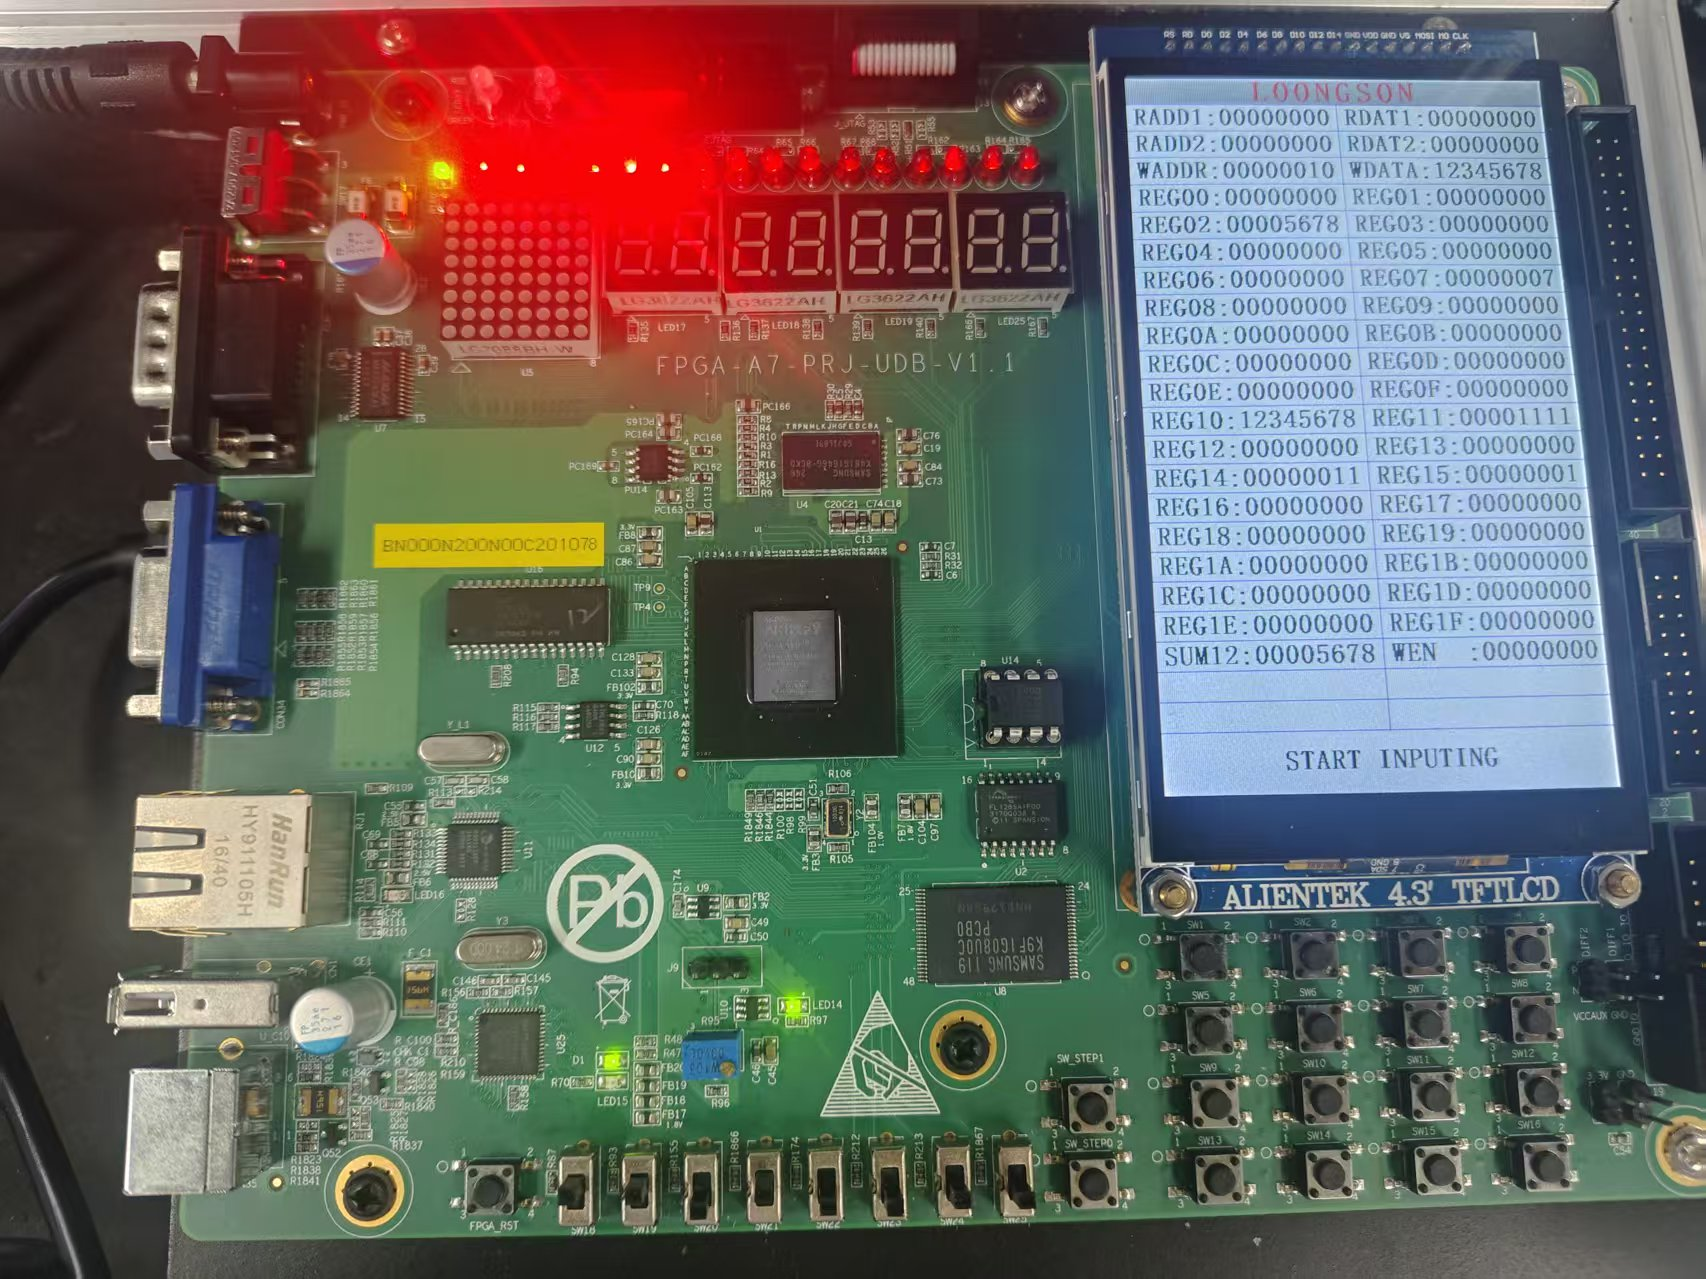
\includegraphics[width=0.8\textwidth]{board1.jpg}
    \caption{实验箱上板验证：读32位，把12345678读入REG10}
    \label{fig:board_photo1}
\end{figure}

\begin{figure}[H]
    \centering
    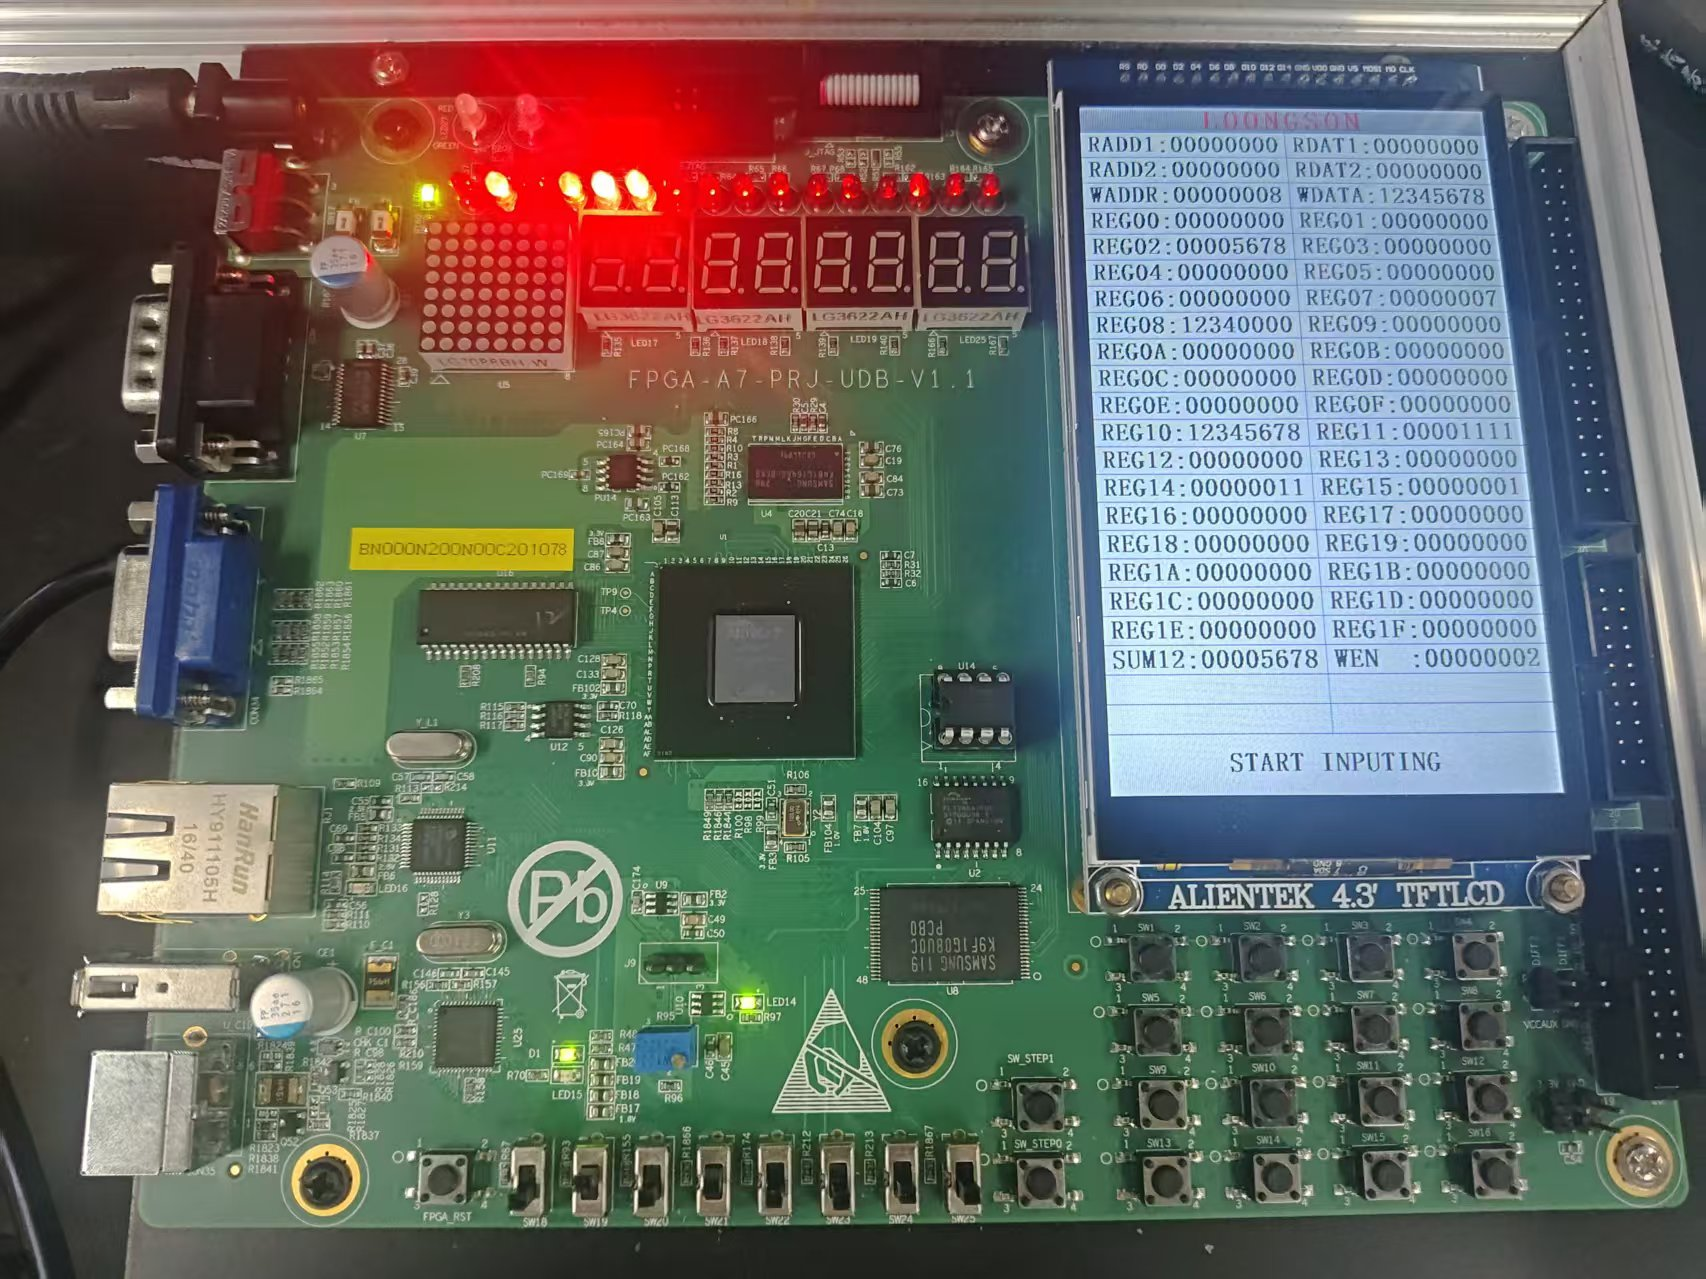
\includegraphics[width=0.8\textwidth]{board2.jpg}
    \caption{实验箱上板验证：读写高16位,把12345678读入REG08}
    \label{fig:board_photo2}
\end{figure}

\begin{figure}[H]
    \centering
    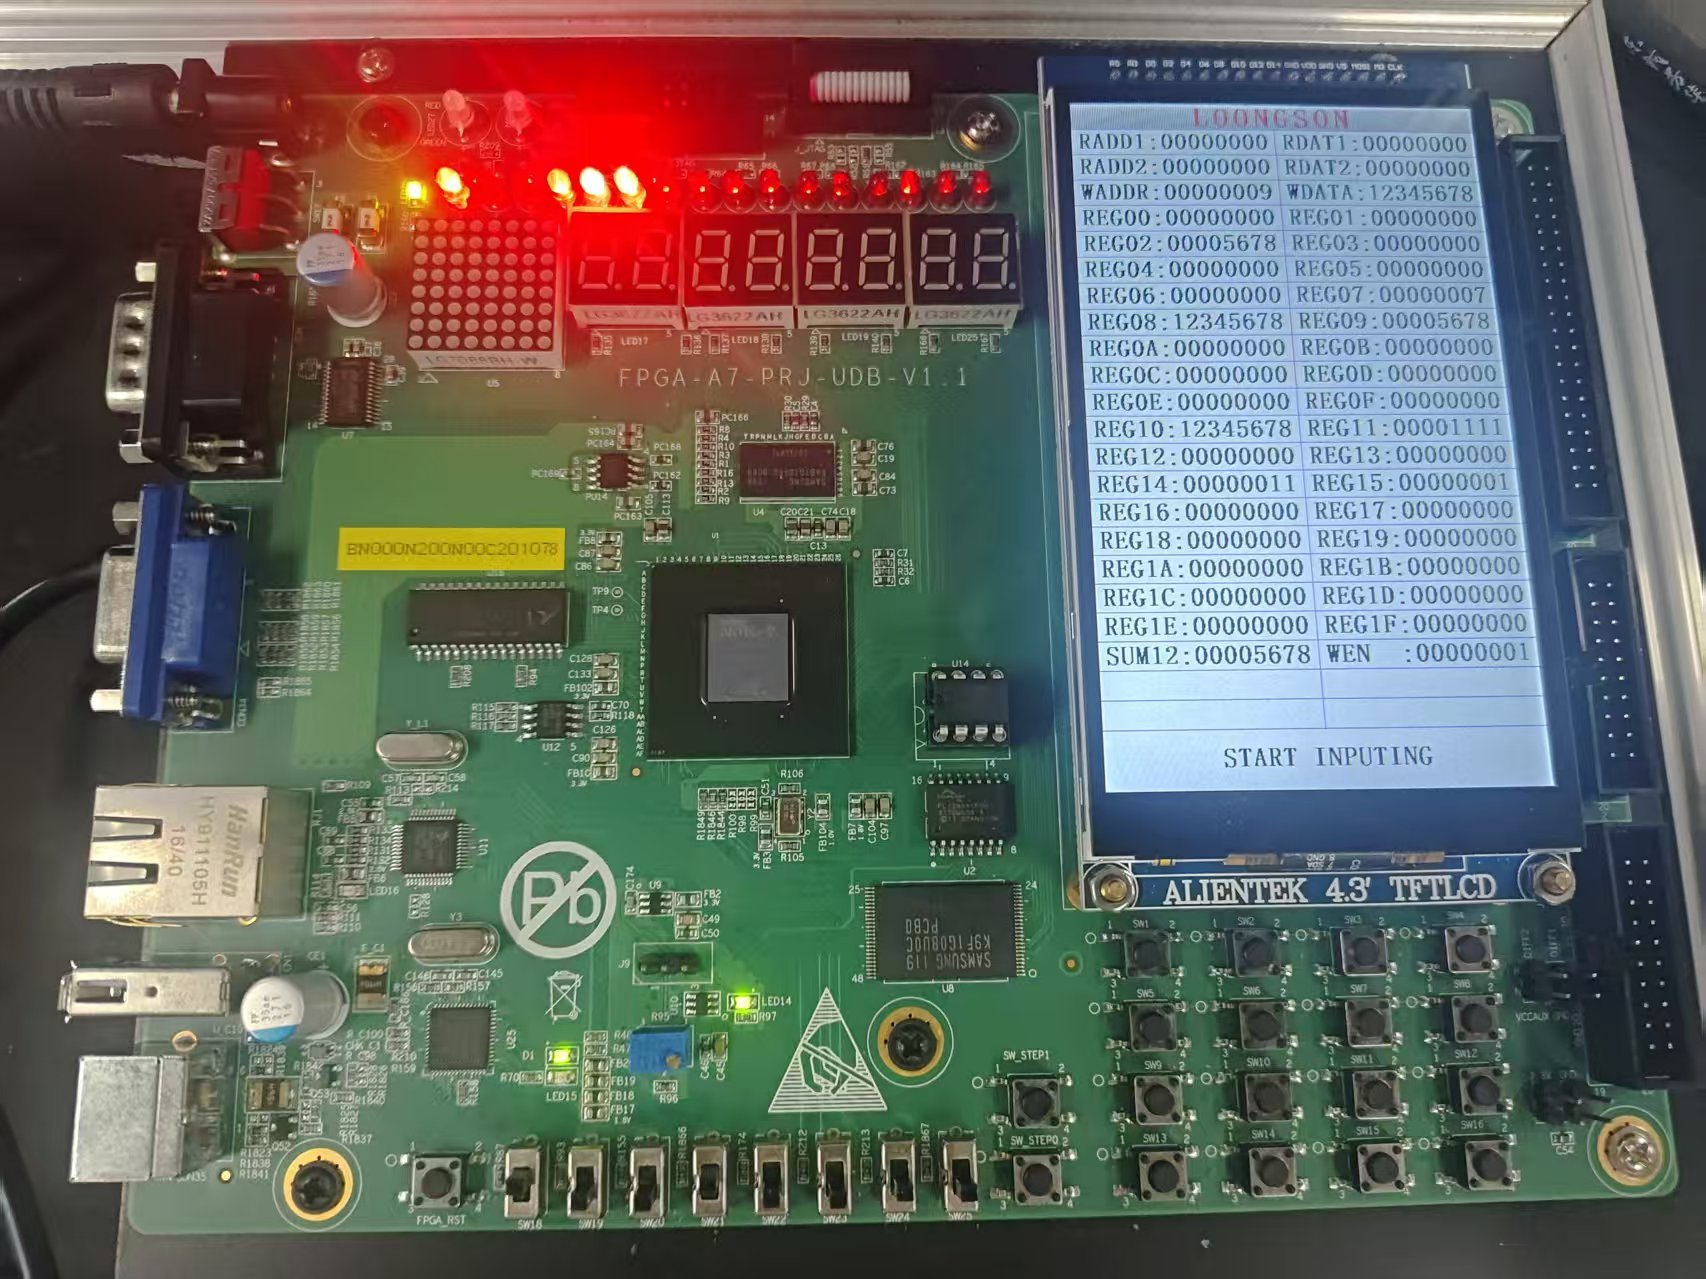
\includegraphics[width=0.8\textwidth]{board3.jpg}
    \caption{实验箱上板验证：读写低16位,把12345678读入REG09}
    \label{fig:board_photo3}
\end{figure}

\begin{figure}[H]
    \centering
    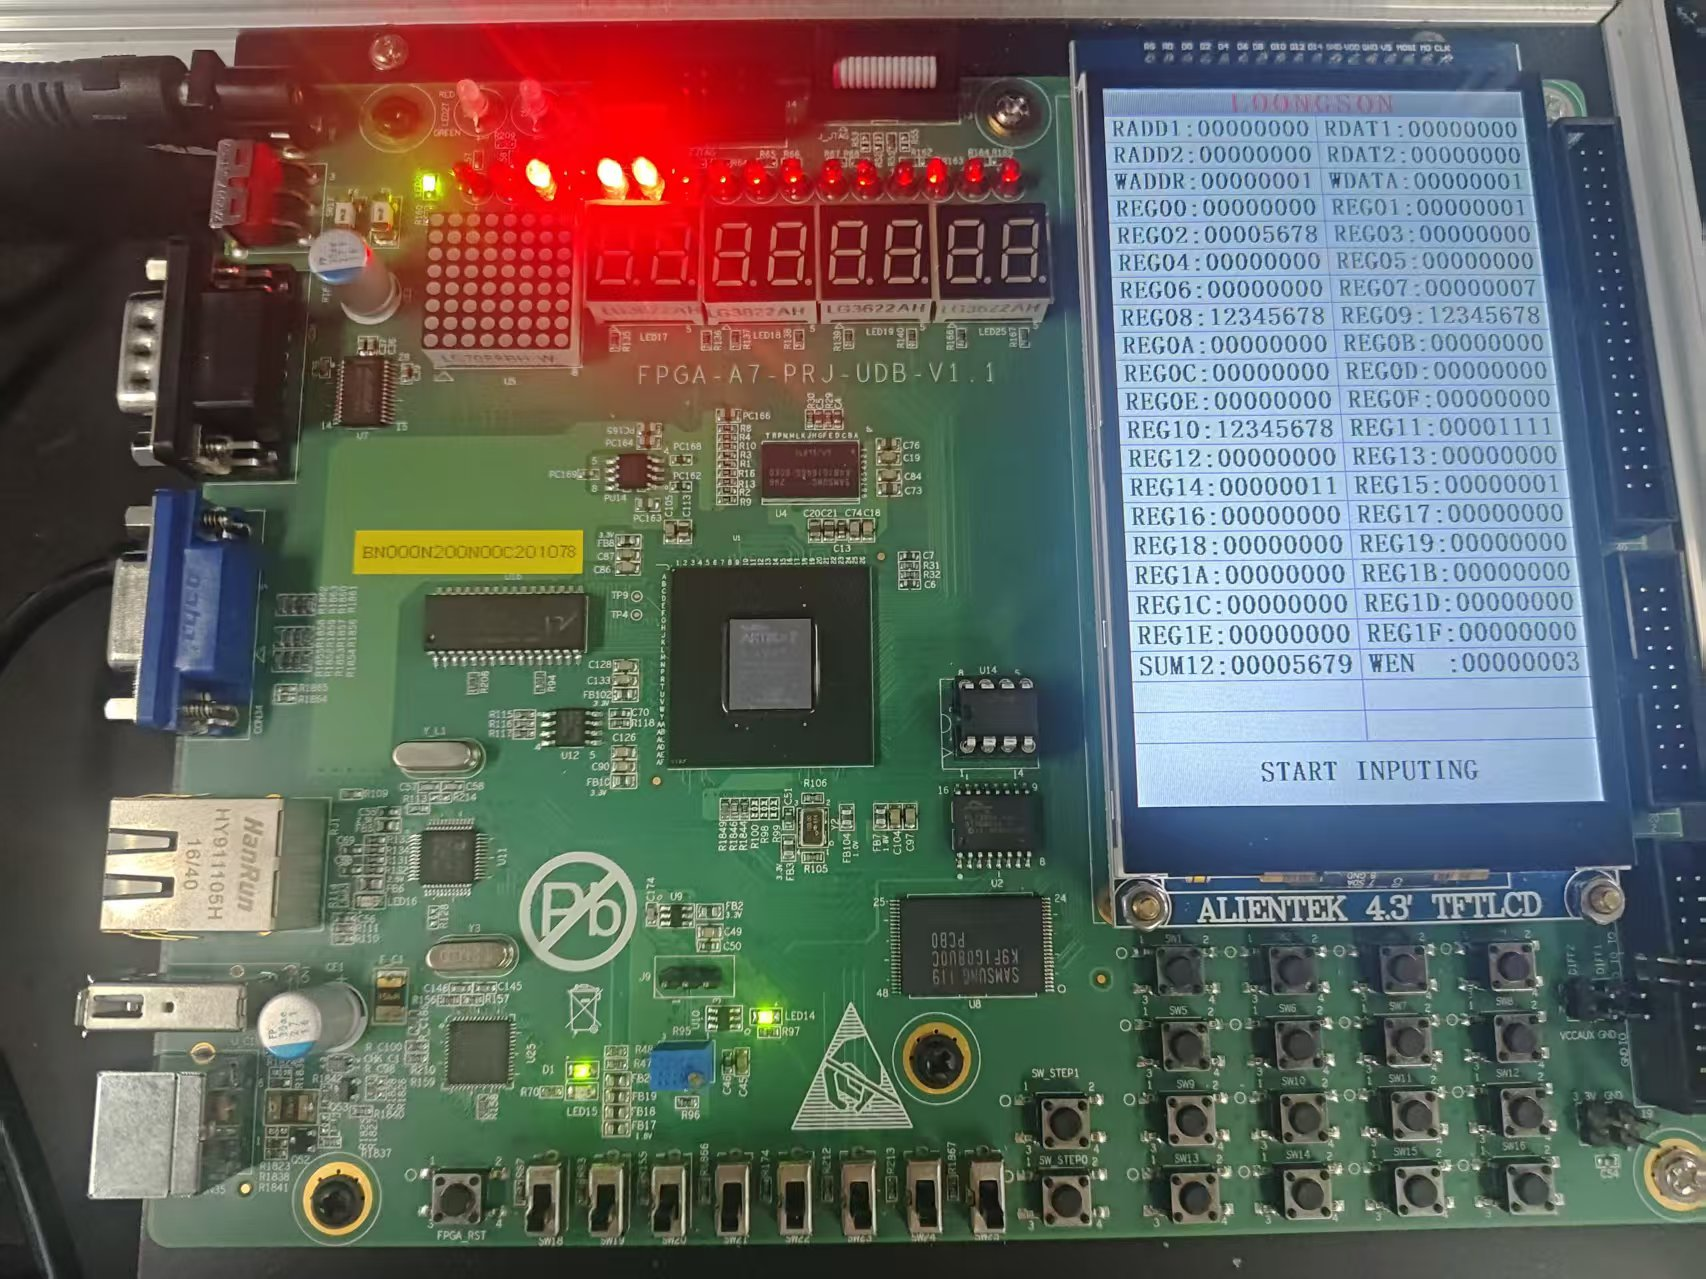
\includegraphics[width=0.8\textwidth]{board4.jpg}
    \caption{实验箱上板验证：检查sum专用寄存器的功能,REG1+REG2}
    \label{fig:board_photo4}
\end{figure}

\section{实验收获}
\begin{itemize}
   \item 熟悉了寄存器堆的设计、读写控制
   \item 实现了通过选择信号读写高低位，用一个更大位宽寄存器的不同段 \\
   模拟多个低位宽寄存器的设计思路，类似于i386的eax, ax, ah, al.
   \item 将寄存器的硬件描述实现和计算机系统基础中对i386 CPU寄存器的结构体模拟联系了起来
\end{itemize}

\section{附：源码目录}
\begin{itemize}
\item \verb|lab3/lab3.srcs/sources_1/new/regfile.v|
\item \verb|lab3/lab3.srcs/sources_1/new/regfile_display.v|
\item \verb|lab3/lab3.srcs/constrs_1/new/regfile.xdc|
\end{itemize}
\end{document}
